% --- Core Variables (with arguments for layer index) ---
% Usage: \hState{l} -> h^(l)_t
\newcommand{\hState}[1]{\mathbf{h}^{(#1)}_t}

% Usage: \Win{l} -> W_in^(l)
\newcommand{\Win}[1]{\mathbf{W}_{\text{in}}^{(#1)}}

% Usage: \Wrec{l} -> W_rec^(l)
\newcommand{\Wrec}[1]{\mathbf{W}_{\text{rec}}^{(#1)}}

% Usage: \Wcyc{l} -> W_cyc^(l)
\newcommand{\Wcyc}[1]{\mathbf{W}_{\text{cyc}}^{(#1)}}


% Usage: \bias{l} -> b^(l)
\newcommand{\bias}[1]{\mathbf{b}^{(#1)}}

% --- Coupling Matrices ---
% Usage: \Cfwd{l} -> C^(l)_forward
\newcommand{\Cfwd}[1]{\mathbf{C}^{(#1)}_{\rightarrow}}
\newcommand{\Cbwd}[1]{\mathbf{C}^{(#1)}_{\leftarrow}}

% --- Total Weight Matrices ---
% Note: Using 'bmatrix' (bracketed matrix) is standard for linear algebra. 
% If you strictly want no brackets, change back to 'matrix'.

\newcommand{\WDeepESN}{
    \begin{bmatrix}
    \Wrec{1} & \mathbf{0} & \cdots & \mathbf{0} \\
    \Win{2} & \Wrec{2} & \cdots & \mathbf{0} \\
    \vdots & \ddots & \ddots & \vdots \\
    \mathbf{0} & \cdots & \Win{L} & \Wrec{L}
    \end{bmatrix}
}

\newcommand{\WtotCycle}{
    \begin{bmatrix}
    \Wrec{1} & \mathbf{0} & \cdots & \mathbf{\Wcyc{1}} \\
    \Wcyc{2} & \Wrec{2} & \cdots & \mathbf{0} \\
    \vdots & \ddots & \ddots & \vdots \\
    \mathbf{0} & \cdots & \Wcyc{L} & \Wrec{L}
    \end{bmatrix}
}

\newcommand{\WtotAntisym}{
    \mathbf{W}_{\text{diag}} +
    \epsilon
    \begin{bmatrix}
    \mathbf{0} & -\Cbwd{1}^\top & \cdots & \mathbf{0} \\
    \Cfwd{1} & \mathbf{0} & \ddots & \vdots \\
    \vdots & \ddots & \ddots & -\Cbwd{L-1}^\top \\
    \mathbf{0} & \cdots & \Cfwd{L-1} & \mathbf{0}
    \end{bmatrix}
}

% !TeX root = ../../main.tex
\label{chap:methodology}
After having discussed all the background concepts and related works, we can now move on to the methodology used in this work
In this chapter we present the idea to treat deep recurrent neural network as \emph{modular deep reservoir} architectures. 
%We will discuss about modularity in RNNs and the two proposed architectures in details. 
Rather than treating reservoir as a monolithic recurrent system, we interpret each layer of the deep reservoir as an independent computational module that processes inputs and exchanges information with other modules through structured interconnections.
The central objective is to study how architectural constraints \ref{...} antisymmetric dynamics with \emph{forward and backward} inter-module coupling, and \ref{...} a \emph{cycle-based} affect stability, memory retention and performance on sequence learning tasks.
\todo{finire di scrivere questo quando avrò un idea di come sara fatta la metodologia}

\section{Modularity in RNNs}
\label{sec:method:modularity}
In dynamical systems theory, a system is said to be \emph{modular} if it can be decomposed into distinct 
subsystems (modules) each of which has its own internal dynamics while also interactting with other modules.
Such composition allows for a complex global behaviour to emerge from the interactions of simpler components.
At the same time, analyzing the system in terms of local module dynamics can provide control on information flow and interpretability benefits.

Modularity has been extensively studied in neuroscience, where large-scale brain networks exhibit modular organization with specialized regions that acts as hubs for information integration.
Empirical studies from Bullmore et al. \cite{bullmore2009complex} have shown that neural systems are composed of densely connected subnetworks that interact globally as a sparse system \todo{che sono connesse in modo sparso forse è meglio?}, supporting
both integration of information and specialized processing 

More generally, studies in complex systems and network dynamics have shown that modular organization 
can enhance robustness by inducing a separation of time scales, such that dynamical processes remain
 confined within subsystems for extended periods before spreading globally. 
 This structure allows perturbations to decay locally and supports stable large-scale 
 dynamics under appropriate stability conditions \cite{Lambiotte_Schaub_2022}.

In this work, we take inspiration from these principles to design deep reservoir architectures, which hierachical structure
can be further enriched with modular interconnections promoting richer dynamics and preserving stability and memory.

\todo{Forse quando parlo in questo modo della modularità nella tesi dovrei anche dire che stiamo trattando le architetture deep "normali" come se fossero    moduli o è già sottinteso?}

\begin{comment}
We consider supervised learning on temporal data.
Given an input sequence $\{\mathbf{u}(t)\}_{t=1}^{T}$ with $\mathbf{u}(t)\in\mathbb{R}^{d_u}$, a reservoir system produces a sequence of hidden states $\{\mathbf{x}(t)\}_{t=1}^{T}$, $\mathbf{x}(t)\in\mathbb{R}^{d_x}$, from which an output sequence $\{\mathbf{y}(t)\}_{t=1}^{T}$ is predicted:
\begin{equation}
    \hat{\mathbf{y}}(t) = \mathbf{W}_{\text{out}} \, \boldsymbol{\phi}(\mathbf{z}(t)) + \mathbf{b}_{\text{out}},
    \label{eq:method:readout}
\end{equation}
where $\mathbf{z}(t)$ is a concatenation of features (e.g., reservoir states across modules and optionally the input), and $\boldsymbol{\phi}(\cdot)$ is a (possibly identity) feature map.
In standard reservoir computing (RC), only the readout parameters $(\mathbf{W}_{\text{out}}, \mathbf{b}_{\text{out}})$ are trained.
\end{comment}
%\clearpage
\section{Deep Modular Reservoirs}
\label{sec:method:deep_modular}
We model a deep reservoir as a composition of $L$ layers or modules. 
Each module $l\in\{1,\dots,L\}$ has state $\mathbf{h}^{(l)}(t)\in\mathbb{R}^{n_l}$ and internal recurrent connectivity $\mathbf{W}^{(l)}$.
The key methodological contribution is to compare two architectures of deep modular reservoirs:

\begin{itemize}
    \item \textbf{Antisymmetric deep reservoir} with \emph{forward and backward} coupling between adjacent modules, designed to promote stable dynamics and improve gradient-free memory propagation.
    \item \textbf{Cycle deep reservoir} where we emply \emph{cycle/ring} recurrent topology, inspired by Simple Cycle Reservoirs (SCR), to provide strong memory traces with minimal parameters.
\end{itemize}

\subsection{Global state and dynamics}
Let $\mathbf{y}(t)$ be the global reservoir state at time $t$ obtained by feeding the input $\mathbf{u}(t)$ into the first module and propagating through the layers.
By stacking the states of all modules, we have the final feature vector used for the readout is made
\begin{equation}
    \mathbf{y}(t) = \begin{bmatrix}
    \mathbf{h}^{(1)}(t) \\
    \mathbf{h}^{(2)}(t) \\
    \vdots \\
    \mathbf{h}^{(L)}(t)
    \end{bmatrix} \in \mathbb{R}^{N}, \quad N = \sum_{l=1}^L n_l.
    \label{eq:method:feature_concat}
\end{equation}
Where $N$ is the total reservoir size and $n_l$ is the size of module $l$.
The global dynamics of the reservoir can be written in the compact form:
obtained after the application of the activation function and leaky integration.

We define the pre-activation vector
\begin{equation}
\mathbf z(t+1) =
\mathbf W_{\text{tot}} \mathbf y(t)
+ \mathbf W_{\text{in}} \mathbf x(t+1)
+ \mathbf b .
\end{equation}

The reservoir state is then updated as
\begin{equation}
\mathbf y(t+1) =
(1-\alpha)\mathbf y(t) + \alpha f(\mathbf z(t+1)).
\end{equation}
\begin{equation}
\mathbf{y}(t+1) = f\left(\mathbf{W}_{\text{tot}} \, \mathbf{y}(t)\right),
\end{equation}
where $f(\cdot)$ acts element-wise on the state vector and
$\mathbf{W}_{\text{tot}} \in \mathbb{R}^{N \times N}$ encodes both intra-module and inter-module connections.


where $\mathbf{W}_{\text{tot}} \in \mathbb{R}^{N \times N}$ is a block matrix that encodes both intra-module and inter-module connections.
For a simple Leaky-ESN with 1 layer, the $\mathbf{W}_{\text{tot}}$ is simply the recurrent weight matrix $\mathbf{W}_{\text{rec}}$ of the reservoir.

So the structure of $\mathbf{W}_{\text{tot}}$ depends on the chosen architecture, a randomly connected module architecture would have 
a block diagonal structure, plus random connections between modules.

\subsubsection{DeepESN as modular system}
In the paper from \cite{GALLICCHIO201787} the authors propose to study what happens when treating modules as a stack, 
hence, in DeepESN architecture with $L$ layers where information is processed hierachically have a matrix for the entire system $W_{\text{DeepESN}}$ in the following form: 

\begin{equation}
    W_{\text{DeepESN}} =\WDeepESN
\end{equation}

Where each block on the diagonal represents the recurrent connections of each module, and the sub-diagonal blocks represent the input connections from the previous layer.
When a single input perturbation is applied, deeper layers retain the perturbation for longer,
 indicating that higher layers capture slower (low‑frequency) temporal components and lower layers capture faster (high‑frequency) components, this is likely due to the fading
 memory effect of the reservoir dynamics.
This indicates that increasing the distance between the input and subsequent layers is crucial for developing a rich spectrum of temporal dynamics
The mechanism of capturing different components of frequency spectrum of the signal is very similar to the one observed in Convolutional Neural Networks (CNNs) for image processing, 
where lower layers capture high-frequency details and higher layers capture low-frequency structures.\todo{forse questo è inutile da dire}

% insert image of deep esn svg
\begin{figure}[ht!]
    \centering
    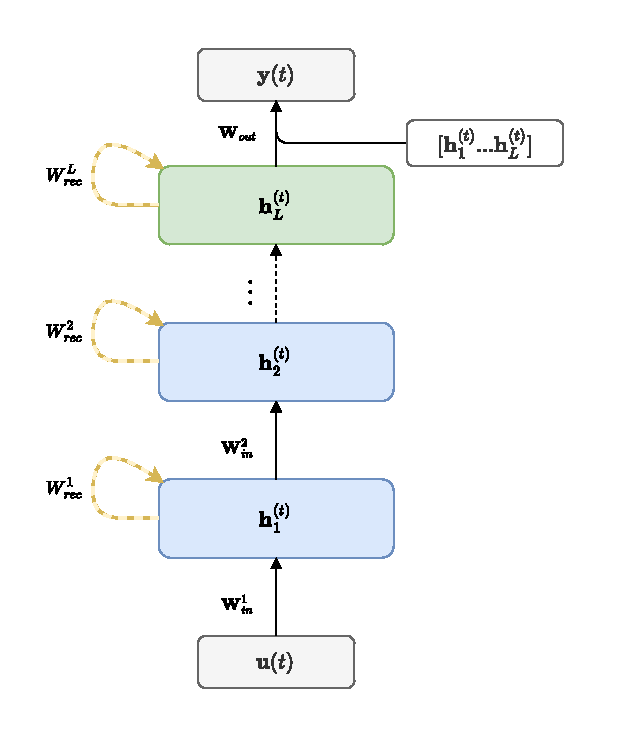
\includegraphics[width=0.5\textwidth]{images/modular_deepesn.pdf}
    \caption{Modular structure of a standard DeepESN. Each layer acts as an independent module with feedforward inter-layer communication.}
\end{figure}

%%%%%%%%%%%%%%%%%%%%%%%%%%%%%%%
\clearpage
\section{Deep Cycle Reservoir}
\label{sec:method:cycle}
The first architecture we propose is inspired to the work of Rodan and Tino \cite{mincomplex}, discussed in sec. \ref{sec:method:cycle}, they
introducing simple and deterministic reservoir models, such as the Simple Cycle Reservoir (SCR), which use a fixed ring topology for the recurrent connections.

\subsection{Motivation}
In a conventional deep ESN, information flows unidirectionally 
from the input through the stacked reservoirs to the readout.
But it lacks a feedback path that might allow higher‑level temporal abstractions
  to influence lower levels. A cyclic deep reservoir introduces a feedback connection 
  from the output of the last reservoir layer back to the first layer.
   The motivation for closing the loop is to allow information processed at deeper layers 
   (capturing longer‑term or low‑frequency features) to inform the processing of new inputs.
    This can enrich the reservoir dynamics and, in principle, improve tasks requiring both short and long‑term memory.


\subsection{Deep Cycle}
We can define the equation for the Deep Cycle Reservoir as follows:

\begin{equation}
    \label{eq:method:cycle_dynamics}
    \begin{cases}
    \mathbf{h}^1{(t)} = (1 - \alpha) \mathbf{h}^1{(t-1)} + \alpha \tanh\left(W_{\text{in}}^{(1)} \mathbf{u{(t)}} + W_{\text{rec}}^{(1)} \mathbf{h}^1{(t-1)} + \math{W}_{cyc}^1 \mathbf{h}^{L}{(t-1)}\right) \\  \\
    \mathbf{h}^l{(t)} = (1 - \alpha) \mathbf{h}^l{(t-1)} + \alpha \tanh\left(W_{\text{in}}^{(l)} \mathbf{u{(t)}} + W_{\text{rec}}^{(l)} \mathbf{h}^l{(t-1)} + \math{W}_{cyc}^l \mathbf{h}^{l-1}{(t-1)}\right) 
    \end{cases}
\end{equation}

We have a (cycle) matrix $W_{cycle}$ with:

\begin{equation}
    W_{cycle}=a\WtotCycle
\end{equation}

Where each $\Wrec{l}$ is scaled by $\rho$ and $\Wcyc{l}$ is initialized as same as recurrent matrices but can have different $\rho$ scaling factor.
The $\rho$ controls the effective spectral radius (for a pure permutation cycle, the eigenvalues lie on the unit circle, and scaling by $\rho$ sets their magnitude).

\subsection{Deep coupling for cycle modules}
We use a forward coupling between modules (and optionally bidirectional coupling as an ablation):
\begin{align}
    \tilde{\mathbf{x}}^{(\ell)}(t+1)
    &= \tanh\!\Big(
        \mathbf{W}^{(\ell)} \mathbf{x}^{(\ell)}(t)
        + \mathbf{W}^{(\ell)}_{\text{in}} \mathbf{h}^{(\ell)}(t+1)
        + \mathbf{C}^{(\ell)} \mathbf{x}^{(\ell-1)}(t)
        + \mathbf{b}^{(\ell)}
    \Big),\\
    \mathbf{x}^{(\ell)}(t+1)
    &= (1-\alpha_\ell)\mathbf{x}^{(\ell)}(t) + \alpha_\ell \tilde{\mathbf{x}}^{(\ell)}(t+1).
\end{align}
This creates a \emph{cycle-based deep reservoir} where each layer has a controlled internal topology and the depth contributes compositional temporal features.


% proof of bounding eigenvlaues
\begin{proof}
    \section{Stability Analysis of Deep Cycle Reservoir via Gershgorin Circle Theorem}

To guarantee the Echo State Property (ESP) and asymptotic stability of the Deep Cycle Reservoir, we analyze the spectral radius of the system's Jacobian. We consider a deep architecture with $L$ layers, where the state update for the $l$-th layer is given by:

\begin{equation}
    \mathbf{h}^{(t)}_l = (1-\alpha)\mathbf{h}^{(t-1)}_l + \alpha \tanh\left( \mathbf{W}_{in}^{(l)}\mathbf{u}^{(t)} + \mathbf{W}_{rec}^{(l)}\mathbf{h}^{(t-1)}_l + \mathbf{W}_{proj}^{prev}\mathbf{h}^{(t-1)}_{prev} \right)
\end{equation}

where $\mathbf{h}_{prev}$ denotes $\mathbf{h}_{l-1}$ for $l > 1$, and $\mathbf{h}_{L}$ for the first layer $l=1$ (closing the cycle).

\subsection{Jacobian Construction}
The effective global weight matrix $\mathbf{J}$ governing the linearized dynamics of the coupled system is a block-circulant-like matrix:

\begin{equation}
    \mathbf{J} = \bigoplus_{l=1}^L \left[ (1-\alpha)\mathbf{I} + \alpha \mathbf{W}_{rec}^{(l)} \right] + \alpha \mathbf{W}_{cycle}
\end{equation}

where $\mathbf{W}_{cycle}$ contains the inter-layer projection blocks $\mathcal{W}_{proj}$ on the sub-diagonal (and top-right).

\subsection{Gershgorin Bound Derivation}
According to the Gershgorin Circle Theorem, the spectrum of $\mathbf{J}$, $\sigma(\mathbf{J})$, is contained within the union of discs $D_i(c_i, R_i)$, where $c_i$ is the diagonal entry and $R_i$ is the sum of the absolute values of the off-diagonal entries of the $i$-th row.

For a neuron $k$ in layer $l$, the center $c_{l,k}$ and radius $R_{l,k}$ are derived as follows:

\begin{enumerate}
    \item \textbf{Center ($c_{l,k}$):} 
    Assuming the recurrent weight matrix $\mathbf{W}_{rec}^{(l)}$ has a zero main diagonal (as in the Simple Cycle Reservoir topology), the diagonal comes solely from the leakage term:
    \begin{equation}
        c_{l,k} = 1 - \alpha
    \end{equation}
    
    \item \textbf{Radius ($R_{l,k}$):}
    The radius is the sum of the magnitudes of incoming weights from two sources: the recurrent connections within layer $l$ and the projection connections from the previous layer in the cycle.
    \begin{equation}
        R_{l,k} = \alpha \left( \sum_{j} |(\mathbf{W}_{rec}^{(l)})_{kj}| + \sum_{p} |(\mathcal{W}_{proj})_{kp}| \right)
    \end{equation}
\end{enumerate}

\subsection{Initialization Specifics}
We evaluate the bound based on the specific initialization schemes used in this work:

\textbf{Case 1: Simple Cycle Reservoir (SCR) Topology} \\
Using the initialization from \texttt{scr.py}, the recurrent matrix $\mathbf{W}_{rec}$ forms a ring where each row has exactly one non-zero element with magnitude $r$. The projection matrix $\mathcal{W}_{proj}$ is initialized (via \texttt{utils.py}) such that the maximum absolute row sum is bounded by a projection strength $\gamma$.
\begin{align}
    \sum_{j} |(\mathbf{W}_{rec}^{(l)})_{kj}| &= r \\
    \sum_{p} |(\mathcal{W}_{proj})_{kp}| &\le \gamma
\end{align}
Substituting these into the Gershgorin radius:
\begin{equation}
    R_{l,k} = \alpha (r + \gamma)
\end{equation}

\textbf{Stability Condition} \\
For stability, we require the spectral radius $\rho(\mathbf{J}) < 1$. By the theorem, it suffices that the largest Gershgorin disc lies entirely within the unit circle. Since the center is at $1-\alpha$ (on the positive real axis), the condition becomes:
\begin{equation}
    c_{l,k} + R_{l,k} < 1 \implies (1 - \alpha) + \alpha(r + \gamma) < 1
\end{equation}

Simplifying the inequality, we obtain the sufficient condition for the Deep Cycle Reservoir:
\begin{equation}
    \boxed{r + \gamma < 1}
\end{equation}

This result proves that in a Deep Cycle architecture initialized with SCR blocks, the sum of the recurrent weight $r$ and the effective projection strength $\gamma$ must be strictly less than 1 to theoretically guarantee the Echo State Property via Gershgorin analysis.
\end{proof}


\section{Deep Antisymmetric Reservoir}
\label{sec:method:antisymmetric}

\subsection{Motivation}
Antisymmetric (or skew-symmetric) connectivity can constrain the dynamics in a way that mitigates exploding trajectories.
Intuitively, purely antisymmetric linear dynamics preserve energy in continuous time; in practice, discrete-time nonlinear systems may still benefit from the improved conditioning and stability induced by such constraints.

\subsection{Module dynamics}
For module $\ell$, we use a leaky update of the form:
\begin{align}
    \tilde{\mathbf{x}}^{(\ell)}(t+1)
    &= \tanh\!\Big(
        \mathbf{W}^{(\ell)} \mathbf{x}^{(\ell)}(t)
        + \mathbf{W}^{(\ell)}_{\text{in}} \mathbf{h}^{(\ell)}(t+1)
        + \mathbf{C}^{(\ell)}_{\rightarrow}\mathbf{x}^{(\ell-1)}(t)
        + \mathbf{C}^{(\ell)}_{\leftarrow}\mathbf{x}^{(\ell+1)}(t)
        + \mathbf{b}^{(\ell)}
    \Big), \label{eq:method:antisym_pre}\\
    \mathbf{x}^{(\ell)}(t+1)
    &= (1-\alpha_\ell)\mathbf{x}^{(\ell)}(t) + \alpha_\ell \tilde{\mathbf{x}}^{(\ell)}(t+1),
    \label{eq:method:antisym_leak}
\end{align}
where $\alpha_\ell\in(0,1]$ is a leak rate.
We set $\mathbf{x}^{(0)}(t)\equiv \mathbf{0}$ and $\mathbf{x}^{(L+1)}(t)\equiv \mathbf{0}$ (or omit missing terms at the boundaries).
The signal $\mathbf{h}^{(\ell)}(t+1)$ is the input to module $\ell$:
\begin{equation}
    \mathbf{h}^{(1)}(t+1) = \mathbf{u}(t+1), \qquad
    \mathbf{h}^{(\ell)}(t+1) = \mathbf{x}^{(\ell-1)}(t) \ \text{for}\ \ell\ge 2
\end{equation}
(or an alternative design depending on the experiment; this is explicitly controlled in ablations).

\subsection{Antisymmetric parametrization}
To construct an antisymmetric recurrent matrix, we sample a raw matrix $\mathbf{A}^{(\ell)}$ and set:
\begin{equation}
    \mathbf{W}^{(\ell)} = \gamma_\ell \left(\mathbf{A}^{(\ell)} - \mathbf{A}^{(\ell)\top}\right),
    \label{eq:method:antisym_W}
\end{equation}
where $\gamma_\ell>0$ controls the effective scale (optionally followed by spectral normalization).
Coupling matrices $\mathbf{C}^{(\ell)}_{\rightarrow}$ (forward) and $\mathbf{C}^{(\ell)}_{\leftarrow}$ (backward) are initialized as sparse random matrices and rescaled by coupling strengths $c_{\rightarrow}$ and $c_{\leftarrow}$.
This yields a \emph{bidirectionally coupled} deep reservoir, enabling information flow from lower to higher modules and feedback from higher to lower modules.

\subsection{Coupling ablations}
To isolate the effect of bidirectionality, we evaluate:
\begin{itemize}
    \item \textbf{Forward-only}: $\mathbf{C}^{(\ell)}_{\leftarrow}=\mathbf{0}$.
    \item \textbf{Backward-only}: $\mathbf{C}^{(\ell)}_{\rightarrow}=\mathbf{0}$.
    \item \textbf{Bidirectional}: both terms active.
\end{itemize}

\section{Initialization and Hyperparameters}
\label{sec:method:hyperparams}

Across both architectures, we control:
\begin{itemize}
    \item \textbf{Module sizes} $\{n_\ell\}_{\ell=1}^L$ and depth $L$.
    \item \textbf{Leak rates} $\alpha_\ell$ (shared or per-layer).
    \item \textbf{Input scaling} for $\mathbf{W}^{(\ell)}_{\text{in}}$ and coupling scaling for $\mathbf{C}$ matrices.
    \item \textbf{Spectral scaling}: $\gamma_\ell$ for antisymmetric modules or $\rho_\ell$ for cycle modules.
    \item \textbf{Readout regularization} $\lambda$ in Eq.~\eqref{eq:method:ridge}.
\end{itemize}

All random matrices are initialized from zero-mean distributions (Gaussian or uniform) and then rescaled to match target norms/sparsity.
We repeat experiments across multiple random seeds to estimate variance.

\section{Training and Evaluation Protocol}
\label{sec:method:protocol}

\subsection{Data preprocessing}
Inputs are standardized per feature (mean $0$, variance $1$) when applicable.
For classification tasks, targets are one-hot encoded; for regression, targets are optionally standardized and rescaled back for reporting.

\subsection{Washout}
To reduce dependence on the initial state, we discard an initial \emph{washout} segment of length $T_{\text{w}}$.
Only states $\{\mathbf{z}(t)\}_{t=T_{\text{w}}+1}^{T}$ are used for training and evaluation.

\subsection{Metrics}
We report:
\begin{itemize}
    \item \textbf{Classification}: accuracy (and macro-F1 when class imbalance is present).
    \item \textbf{Regression}: mean squared error (MSE) and normalized RMSE (when appropriate).
    \item \textbf{Memory}: memory capacity (MC) or task-specific memory measures when included in the benchmark suite.
\end{itemize}

\subsection{Baselines}
We compare the proposed architectures against:
\begin{itemize}
    \item A standard single-layer ESN with comparable total state dimension.
    \item A deep ESN with forward-only coupling (when the proposed model is bidirectional).
    \item A structured SCR-like single module (when evaluating the benefit of depth).
\end{itemize}

\section{Ablation Studies}
\label{sec:method:ablations}

We perform controlled ablations to attribute performance gains:
\begin{enumerate}
    \item \textbf{Coupling directionality}: forward vs backward vs bidirectional.
    \item \textbf{Structure vs randomness}: antisymmetric/cycle $\mathbf{W}^{(\ell)}$ vs dense random $\mathbf{W}^{(\ell)}$ under matched scaling.
    \item \textbf{Depth vs width}: varying $L$ while keeping total state size $\sum_\ell n_\ell$ fixed.
    \item \textbf{Readout features}: last-layer-only vs concatenation across layers (Eq.~\eqref{eq:method:feature_concat}).
\end{enumerate}

\section{Implementation Notes}
\label{sec:method:implementation}

All models are implemented in Python with vectorized state updates.
For reproducibility, experiments log the random seed, hyperparameters, and the exact dataset split.
Unless otherwise specified, only the linear readout is trained, enabling efficient training via closed-form ridge regression (Eq.~\eqref{eq:method:ridge}).

\section{Summary}
\label{sec:method:summary}

The methodology evaluates two modular deep reservoir families:
(1) antisymmetric modules with bidirectional coupling to study stability and information flow,
and (2) cycle-based (SCR-like) modules to study the effect of strong structural priors.
Both are trained with identical readout procedures and compared under matched experimental controls to isolate architectural effects.

\subsection{Modular Interpretation of Deep Reservoir Architectures}

All architectures considered in this work can be interpreted as \emph{modular dynamical systems}, where each reservoir layer acts as an autonomous computational module.
Each module consists of a fixed number of recurrent units that process incoming signals and exchange information with other modules according to a prescribed connectivity pattern.

Let each module $l \in \{1,\dots,L\}$ be associated with a state vector
$\mathbf{h}^{(l)}_t \in \mathbb{R}^{N_l}$, where $N_l$ is the number of units in the layer.
Modules interact exclusively through linear projections of their internal states, while nonlinear processing occurs locally within each module.

This modular view allows the architecture to be analyzed in terms of structured interconnections between subsystems, rather than as a monolithic recurrent network.

\subsection{Standard DeepESN: Hierarchical Modularity}

In a standard DeepESN without cyclic or antisymmetric connections, information flows strictly forward across layers.
The global recurrent matrix has a \emph{block lower-triangular} structure:
\begin{equation}
\mathbf{W}_{\text{tot}} =
\begin{bmatrix}
\mathbf{W}_{rec}^{(1)} & \mathbf{0} & \cdots & \mathbf{0} \\
\mathbf{W}_{in}^{(2)} & \mathbf{W}_{rec}^{(2)} & \cdots & \mathbf{0} \\
\vdots & \ddots & \ddots & \vdots \\
\mathbf{0} & \cdots & \mathbf{W}_{in}^{(L)} & \mathbf{W}_{rec}^{(L)}
\end{bmatrix}.
\end{equation}

Each diagonal block represents the internal dynamics of a module, while sub-diagonal blocks model feedforward communication between adjacent modules.
This structure implies that the Jacobian of the system is block lower-triangular, and its spectral radius is governed by the most unstable module.

\begin{figure}[t]
    \centering
    % TODO: insert DeepESN modular diagram
    \fbox{\parbox{0.8\linewidth}{\centering Placeholder for DeepESN modular architecture diagram}}
    \caption{Modular structure of a standard DeepESN. Each layer acts as an independent module with feedforward inter-layer communication.}
    \label{fig:deepesn-modular}
\end{figure}

\subsection{Cycle-Connected DeepESN: Ring Modularity}

When cyclic connectivity is introduced, the modular hierarchy is closed into a ring.
The first module receives feedback from the last module, yielding a block-circulant structure:
\begin{equation}
\mathbf{W}_{\text{tot}} =
\begin{bmatrix}
\mathbf{W}_{rec}^{(1)} & \mathbf{0} & \cdots & \mathbf{P}^{(1)} \\
\mathbf{W}_{in}^{(2)} & \mathbf{W}_{rec}^{(2)} & \cdots & \mathbf{0} \\
\vdots & \ddots & \ddots & \vdots \\
\mathbf{0} & \cdots & \mathbf{W}_{in}^{(L)} & \mathbf{W}_{rec}^{(L)}
\end{bmatrix},
\end{equation}
where $\mathbf{P}^{(1)}$ denotes the projection from the last module to the first.

This ring topology removes the strict feedforward ordering of modules and enables global feedback across depth, significantly altering the spectrum of $\mathbf{W}_{\text{tot}}$ and the resulting memory dynamics.

\begin{figure}[t]
    \centering
    % TODO: insert Cycle DeepESN diagram
    \fbox{\parbox{0.8\linewidth}{\centering Placeholder for cyclic modular architecture diagram}}
    \caption{Cycle-connected DeepESN. Modules are arranged in a ring topology, enabling feedback across depth.}
    \label{fig:cycle-modular}
\end{figure}

\subsection{Antisymmetric Modular Coupling}

In the antisymmetric architecture, modules interact bidirectionally with neighboring modules through antisymmetric couplings.
The global recurrent matrix can be written as:
\begin{equation}
\mathbf{W}_{\text{tot}} =
\mathbf{W}_{\text{diag}} +
\epsilon
\begin{bmatrix}
\mathbf{0} & -\mathbf{C}^\top & \cdots & \mathbf{0} \\
\mathbf{C} & \mathbf{0} & \ddots & \vdots \\
\vdots & \ddots & \ddots & -\mathbf{C}^\top \\
\mathbf{0} & \cdots & \mathbf{C} & \mathbf{0}
\end{bmatrix}
- \gamma \mathbf{I},
\end{equation}
where $\mathbf{W}_{\text{diag}}$ contains the block-diagonal recurrent matrices of each module.

This construction enforces near-skew-symmetry of the inter-module dynamics, which theoretically promotes marginal stability and critical behavior.
Each module remains locally nonlinear, while global interactions preserve structured energy exchange across layers.

\begin{figure}[t]
    \centering
    % TODO: insert antisymmetric modular diagram
    \fbox{\parbox{0.8\linewidth}{\centering Placeholder for antisymmetric modular architecture diagram}}
    \caption{Antisymmetric modular coupling across layers. Each module exchanges state information with its neighbors through skew-symmetric projections.}
    \label{fig:antisymmetric-modular}
\end{figure}

\subsection{Extension to Randomized Oscillators Networks}

The same modular decomposition applies to RON and DeepRON architectures.
Each layer represents a second-order dynamical module, and the global system can be expressed by stacking first-order representations of position and velocity states.

Inter-module connectivity (feedforward, cyclic, or antisymmetric) affects only the linear coupling terms, while local oscillator dynamics remain unchanged.
This allows a direct comparison between discrete-time (ESN) and continuous-time-inspired (RON) reservoirs under a unified modular framework.
